% Options for packages loaded elsewhere
\PassOptionsToPackage{unicode}{hyperref}
\PassOptionsToPackage{hyphens}{url}
\PassOptionsToPackage{dvipsnames,svgnames,x11names}{xcolor}
%
\documentclass[
  letterpaper,
  DIV=11,
  numbers=noendperiod]{scrreprt}

\usepackage{amsmath,amssymb}
\usepackage{iftex}
\ifPDFTeX
  \usepackage[T1]{fontenc}
  \usepackage[utf8]{inputenc}
  \usepackage{textcomp} % provide euro and other symbols
\else % if luatex or xetex
  \usepackage{unicode-math}
  \defaultfontfeatures{Scale=MatchLowercase}
  \defaultfontfeatures[\rmfamily]{Ligatures=TeX,Scale=1}
\fi
\usepackage{lmodern}
\ifPDFTeX\else  
    % xetex/luatex font selection
\fi
% Use upquote if available, for straight quotes in verbatim environments
\IfFileExists{upquote.sty}{\usepackage{upquote}}{}
\IfFileExists{microtype.sty}{% use microtype if available
  \usepackage[]{microtype}
  \UseMicrotypeSet[protrusion]{basicmath} % disable protrusion for tt fonts
}{}
\makeatletter
\@ifundefined{KOMAClassName}{% if non-KOMA class
  \IfFileExists{parskip.sty}{%
    \usepackage{parskip}
  }{% else
    \setlength{\parindent}{0pt}
    \setlength{\parskip}{6pt plus 2pt minus 1pt}}
}{% if KOMA class
  \KOMAoptions{parskip=half}}
\makeatother
\usepackage{xcolor}
\setlength{\emergencystretch}{3em} % prevent overfull lines
\setcounter{secnumdepth}{-\maxdimen} % remove section numbering
% Make \paragraph and \subparagraph free-standing
\ifx\paragraph\undefined\else
  \let\oldparagraph\paragraph
  \renewcommand{\paragraph}[1]{\oldparagraph{#1}\mbox{}}
\fi
\ifx\subparagraph\undefined\else
  \let\oldsubparagraph\subparagraph
  \renewcommand{\subparagraph}[1]{\oldsubparagraph{#1}\mbox{}}
\fi

\usepackage{color}
\usepackage{fancyvrb}
\newcommand{\VerbBar}{|}
\newcommand{\VERB}{\Verb[commandchars=\\\{\}]}
\DefineVerbatimEnvironment{Highlighting}{Verbatim}{commandchars=\\\{\}}
% Add ',fontsize=\small' for more characters per line
\usepackage{framed}
\definecolor{shadecolor}{RGB}{241,243,245}
\newenvironment{Shaded}{\begin{snugshade}}{\end{snugshade}}
\newcommand{\AlertTok}[1]{\textcolor[rgb]{0.68,0.00,0.00}{#1}}
\newcommand{\AnnotationTok}[1]{\textcolor[rgb]{0.37,0.37,0.37}{#1}}
\newcommand{\AttributeTok}[1]{\textcolor[rgb]{0.40,0.45,0.13}{#1}}
\newcommand{\BaseNTok}[1]{\textcolor[rgb]{0.68,0.00,0.00}{#1}}
\newcommand{\BuiltInTok}[1]{\textcolor[rgb]{0.00,0.23,0.31}{#1}}
\newcommand{\CharTok}[1]{\textcolor[rgb]{0.13,0.47,0.30}{#1}}
\newcommand{\CommentTok}[1]{\textcolor[rgb]{0.37,0.37,0.37}{#1}}
\newcommand{\CommentVarTok}[1]{\textcolor[rgb]{0.37,0.37,0.37}{\textit{#1}}}
\newcommand{\ConstantTok}[1]{\textcolor[rgb]{0.56,0.35,0.01}{#1}}
\newcommand{\ControlFlowTok}[1]{\textcolor[rgb]{0.00,0.23,0.31}{#1}}
\newcommand{\DataTypeTok}[1]{\textcolor[rgb]{0.68,0.00,0.00}{#1}}
\newcommand{\DecValTok}[1]{\textcolor[rgb]{0.68,0.00,0.00}{#1}}
\newcommand{\DocumentationTok}[1]{\textcolor[rgb]{0.37,0.37,0.37}{\textit{#1}}}
\newcommand{\ErrorTok}[1]{\textcolor[rgb]{0.68,0.00,0.00}{#1}}
\newcommand{\ExtensionTok}[1]{\textcolor[rgb]{0.00,0.23,0.31}{#1}}
\newcommand{\FloatTok}[1]{\textcolor[rgb]{0.68,0.00,0.00}{#1}}
\newcommand{\FunctionTok}[1]{\textcolor[rgb]{0.28,0.35,0.67}{#1}}
\newcommand{\ImportTok}[1]{\textcolor[rgb]{0.00,0.46,0.62}{#1}}
\newcommand{\InformationTok}[1]{\textcolor[rgb]{0.37,0.37,0.37}{#1}}
\newcommand{\KeywordTok}[1]{\textcolor[rgb]{0.00,0.23,0.31}{#1}}
\newcommand{\NormalTok}[1]{\textcolor[rgb]{0.00,0.23,0.31}{#1}}
\newcommand{\OperatorTok}[1]{\textcolor[rgb]{0.37,0.37,0.37}{#1}}
\newcommand{\OtherTok}[1]{\textcolor[rgb]{0.00,0.23,0.31}{#1}}
\newcommand{\PreprocessorTok}[1]{\textcolor[rgb]{0.68,0.00,0.00}{#1}}
\newcommand{\RegionMarkerTok}[1]{\textcolor[rgb]{0.00,0.23,0.31}{#1}}
\newcommand{\SpecialCharTok}[1]{\textcolor[rgb]{0.37,0.37,0.37}{#1}}
\newcommand{\SpecialStringTok}[1]{\textcolor[rgb]{0.13,0.47,0.30}{#1}}
\newcommand{\StringTok}[1]{\textcolor[rgb]{0.13,0.47,0.30}{#1}}
\newcommand{\VariableTok}[1]{\textcolor[rgb]{0.07,0.07,0.07}{#1}}
\newcommand{\VerbatimStringTok}[1]{\textcolor[rgb]{0.13,0.47,0.30}{#1}}
\newcommand{\WarningTok}[1]{\textcolor[rgb]{0.37,0.37,0.37}{\textit{#1}}}

\providecommand{\tightlist}{%
  \setlength{\itemsep}{0pt}\setlength{\parskip}{0pt}}\usepackage{longtable,booktabs,array}
\usepackage{calc} % for calculating minipage widths
% Correct order of tables after \paragraph or \subparagraph
\usepackage{etoolbox}
\makeatletter
\patchcmd\longtable{\par}{\if@noskipsec\mbox{}\fi\par}{}{}
\makeatother
% Allow footnotes in longtable head/foot
\IfFileExists{footnotehyper.sty}{\usepackage{footnotehyper}}{\usepackage{footnote}}
\makesavenoteenv{longtable}
\usepackage{graphicx}
\makeatletter
\def\maxwidth{\ifdim\Gin@nat@width>\linewidth\linewidth\else\Gin@nat@width\fi}
\def\maxheight{\ifdim\Gin@nat@height>\textheight\textheight\else\Gin@nat@height\fi}
\makeatother
% Scale images if necessary, so that they will not overflow the page
% margins by default, and it is still possible to overwrite the defaults
% using explicit options in \includegraphics[width, height, ...]{}
\setkeys{Gin}{width=\maxwidth,height=\maxheight,keepaspectratio}
% Set default figure placement to htbp
\makeatletter
\def\fps@figure{htbp}
\makeatother

\usepackage{booktabs}
\usepackage{longtable}
\usepackage{array}
\usepackage{multirow}
\usepackage{wrapfig}
\usepackage{float}
\usepackage{colortbl}
\usepackage{pdflscape}
\usepackage{tabu}
\usepackage{threeparttable}
\usepackage{threeparttablex}
\usepackage[normalem]{ulem}
\usepackage{makecell}
\usepackage{xcolor}
\usepackage{siunitx}

  \newcolumntype{d}{S[
    input-open-uncertainty=,
    input-close-uncertainty=,
    parse-numbers = false,
    table-align-text-pre=false,
    table-align-text-post=false
  ]}
  
\KOMAoption{captions}{tableheading}
\makeatletter
\@ifpackageloaded{tcolorbox}{}{\usepackage[skins,breakable]{tcolorbox}}
\@ifpackageloaded{fontawesome5}{}{\usepackage{fontawesome5}}
\definecolor{quarto-callout-color}{HTML}{909090}
\definecolor{quarto-callout-note-color}{HTML}{0758E5}
\definecolor{quarto-callout-important-color}{HTML}{CC1914}
\definecolor{quarto-callout-warning-color}{HTML}{EB9113}
\definecolor{quarto-callout-tip-color}{HTML}{00A047}
\definecolor{quarto-callout-caution-color}{HTML}{FC5300}
\definecolor{quarto-callout-color-frame}{HTML}{acacac}
\definecolor{quarto-callout-note-color-frame}{HTML}{4582ec}
\definecolor{quarto-callout-important-color-frame}{HTML}{d9534f}
\definecolor{quarto-callout-warning-color-frame}{HTML}{f0ad4e}
\definecolor{quarto-callout-tip-color-frame}{HTML}{02b875}
\definecolor{quarto-callout-caution-color-frame}{HTML}{fd7e14}
\makeatother
\makeatletter
\makeatother
\makeatletter
\makeatother
\makeatletter
\@ifpackageloaded{caption}{}{\usepackage{caption}}
\AtBeginDocument{%
\ifdefined\contentsname
  \renewcommand*\contentsname{Table of contents}
\else
  \newcommand\contentsname{Table of contents}
\fi
\ifdefined\listfigurename
  \renewcommand*\listfigurename{List of Figures}
\else
  \newcommand\listfigurename{List of Figures}
\fi
\ifdefined\listtablename
  \renewcommand*\listtablename{List of Tables}
\else
  \newcommand\listtablename{List of Tables}
\fi
\ifdefined\figurename
  \renewcommand*\figurename{Figure}
\else
  \newcommand\figurename{Figure}
\fi
\ifdefined\tablename
  \renewcommand*\tablename{Table}
\else
  \newcommand\tablename{Table}
\fi
}
\@ifpackageloaded{float}{}{\usepackage{float}}
\floatstyle{ruled}
\@ifundefined{c@chapter}{\newfloat{codelisting}{h}{lop}}{\newfloat{codelisting}{h}{lop}[chapter]}
\floatname{codelisting}{Listing}
\newcommand*\listoflistings{\listof{codelisting}{List of Listings}}
\makeatother
\makeatletter
\@ifpackageloaded{caption}{}{\usepackage{caption}}
\@ifpackageloaded{subcaption}{}{\usepackage{subcaption}}
\makeatother
\makeatletter
\@ifpackageloaded{tcolorbox}{}{\usepackage[skins,breakable]{tcolorbox}}
\makeatother
\makeatletter
\@ifundefined{shadecolor}{\definecolor{shadecolor}{rgb}{.97, .97, .97}}
\makeatother
\makeatletter
\makeatother
\makeatletter
\makeatother
\makeatletter
\@ifpackageloaded{tikz}{}{\usepackage{tikz}}
\makeatother
        \newcommand*\circled[1]{\tikz[baseline=(char.base)]{
          \node[shape=circle,draw,inner sep=1pt] (char) {{\scriptsize#1}};}}  
                  
\ifLuaTeX
  \usepackage{selnolig}  % disable illegal ligatures
\fi
\IfFileExists{bookmark.sty}{\usepackage{bookmark}}{\usepackage{hyperref}}
\IfFileExists{xurl.sty}{\usepackage{xurl}}{} % add URL line breaks if available
\urlstyle{same} % disable monospaced font for URLs
\hypersetup{
  pdftitle={8 単回帰分析},
  colorlinks=true,
  linkcolor={blue},
  filecolor={Maroon},
  citecolor={Blue},
  urlcolor={Blue},
  pdfcreator={LaTeX via pandoc}}

\title{8 単回帰分析}
\author{}
\date{}

\begin{document}
\maketitle
\ifdefined\Shaded\renewenvironment{Shaded}{\begin{tcolorbox}[frame hidden, enhanced, boxrule=0pt, sharp corners, interior hidden, breakable, borderline west={3pt}{0pt}{shadecolor}]}{\end{tcolorbox}}\fi

\hypertarget{annotated-cell-1}{%
\label{annotated-cell-1}}%
\begin{Shaded}
\begin{Highlighting}[]
\FunctionTok{rm}\NormalTok{(}\AttributeTok{list=}\FunctionTok{ls}\NormalTok{()); }\FunctionTok{gc}\NormalTok{();  }\FunctionTok{gc}\NormalTok{(); }\CommentTok{\#\textless{}1\textgreater{}}
\ControlFlowTok{if}\NormalTok{ (}\SpecialCharTok{!}\FunctionTok{require}\NormalTok{(}\StringTok{"pacman"}\NormalTok{)) }\FunctionTok{install.packages}\NormalTok{(}\StringTok{"pacman"}\NormalTok{) }\CommentTok{\#\textless{}2\textgreater{}}
\NormalTok{pacman}\SpecialCharTok{::}\FunctionTok{p\_load}\NormalTok{(tidyverse, magrittr,estimatr,car,modelsummary,ggrepel,patchwork) }\CommentTok{\#\textless{}3\textgreater{}}
\end{Highlighting}
\end{Shaded}

\begin{description}
\tightlist
\item[\circled{1}]
前の作業など,rのメモリに入っているものをリセットするコマンド
\item[\circled{2}]
パッケージ管理用のパッケージである\texttt{pacman}が入っていない場合はインストール
\item[\circled{3}]
複数のパッケージを一度に呼び出す
\end{description}

データの読み込み

\begin{Shaded}
\begin{Highlighting}[]
\NormalTok{ice4\_1 }\OtherTok{\textless{}{-}} \FunctionTok{read\_csv}\NormalTok{(}\StringTok{"data/ice4\_1.csv"}\NormalTok{)}
\NormalTok{ice4\_1}
\end{Highlighting}
\end{Shaded}

\begin{verbatim}
# A tibble: 20 x 3
     num  kion kyaku
   <dbl> <dbl> <dbl>
 1     1    33   382
 2     2    33   324
 3     3    34   338
 4     4    34   317
 5     5    35   341
 6     6    35   360
 7     7    34   339
 8     8    32   329
 9     9    28   218
10    10    35   402
11    11    33   342
12    12    28   205
13    13    32   368
14    14    25   196
15    15    28   304
16    16    30   294
17    17    29   275
18    18    32   336
19    19    34   384
20    20    35   368
\end{verbatim}

気温は\texttt{kion},客数は\texttt{kyaku}という名前になっていることを確認します。

その上でまず,データの散布図と,それにフィットする直線を書いてみます。

\hypertarget{annotated-cell-3}{%
\label{annotated-cell-3}}%
\begin{Shaded}
\begin{Highlighting}[]
\NormalTok{g }\OtherTok{\textless{}{-}} \FunctionTok{ggplot}\NormalTok{(}\AttributeTok{data =}\NormalTok{ ice4\_1, }\CommentTok{\#\textless{}1\textgreater{}}
            \FunctionTok{aes}\NormalTok{(}\AttributeTok{x =}\NormalTok{ kion, }\AttributeTok{y =}\NormalTok{ kyaku) }\CommentTok{\#\textless{}2\textgreater{}}
\NormalTok{            ) }\SpecialCharTok{\%\textgreater{}\%} 
  \SpecialCharTok{+} \FunctionTok{geom\_point}\NormalTok{() }\SpecialCharTok{\%\textgreater{}\%} \CommentTok{\#\textless{}3\textgreater{}}
  \SpecialCharTok{+} \FunctionTok{geom\_smooth}\NormalTok{(}\AttributeTok{method =} \StringTok{"lm"}\NormalTok{,}\AttributeTok{se=}\ConstantTok{FALSE}\NormalTok{) }\CommentTok{\#\textless{}4\textgreater{}}

\FunctionTok{plot}\NormalTok{(g)}
\end{Highlighting}
\end{Shaded}

\begin{description}
\tightlist
\item[\circled{1}]
使うデータを指定
\item[\circled{2}]
x軸とy軸を指定
\item[\circled{3}]
散布図を作成
\item[\circled{4}]
散布図にフィットする直線を書く。方法は,線形モデル(\texttt{lm})
\end{description}

\begin{figure}[H]

{\centering 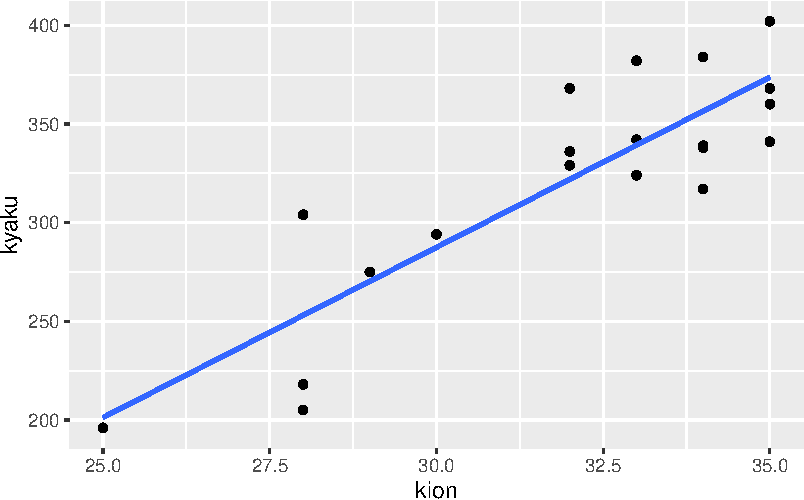
\includegraphics{8_regress_files/figure-pdf/unnamed-chunk-3-1.pdf}

}

\end{figure}

これは,自動で線が引かれていますが,例えばこんな線もあり得そうでもあります。

\hypertarget{annotated-cell-4}{%
\label{annotated-cell-4}}%
\begin{Shaded}
\begin{Highlighting}[]
\NormalTok{g }\OtherTok{\textless{}{-}} \FunctionTok{ggplot}\NormalTok{(}\AttributeTok{data =}\NormalTok{ ice4\_1, }\CommentTok{\#使うデータを指定}
            \FunctionTok{aes}\NormalTok{(}\AttributeTok{x =}\NormalTok{ kion, }\AttributeTok{y =}\NormalTok{ kyaku) }\CommentTok{\#x軸とy軸を指定}
\NormalTok{            ) }\SpecialCharTok{\%\textgreater{}\%} 
  \SpecialCharTok{+} \FunctionTok{geom\_point}\NormalTok{() }\SpecialCharTok{\%\textgreater{}\%} \CommentTok{\#散布図を作成}
  \SpecialCharTok{+} \FunctionTok{geom\_smooth}\NormalTok{(}\AttributeTok{method =} \StringTok{"lm"}\NormalTok{,}\AttributeTok{se=}\ConstantTok{FALSE}\NormalTok{) }\SpecialCharTok{\%\textgreater{}\%} 
  \SpecialCharTok{+} \FunctionTok{geom\_hline}\NormalTok{(}\FunctionTok{aes}\NormalTok{(}\AttributeTok{yintercept=}\DecValTok{320}\NormalTok{),}
               \AttributeTok{color =} \StringTok{"salmon"}\NormalTok{) }\SpecialCharTok{\%\textgreater{}\%} \CommentTok{\#\textless{}1\textgreater{}}
  \SpecialCharTok{+} \FunctionTok{geom\_abline}\NormalTok{(}\AttributeTok{intercept =} \DecValTok{150}\NormalTok{, }\AttributeTok{slope =} \DecValTok{5}\NormalTok{,}
                \AttributeTok{color =} \StringTok{"yellowgreen"}\NormalTok{)}\CommentTok{\#\textless{}2\textgreater{}}

\CommentTok{\#散布図にフィットする直線を書く。方法は,線形モデル(lm)}
\FunctionTok{plot}\NormalTok{(g)}
\end{Highlighting}
\end{Shaded}

\begin{description}
\tightlist
\item[\circled{1}]
高さ320の水平線
\item[\circled{2}]
傾き5,切片150の直線
\end{description}

\begin{figure}[H]

{\centering 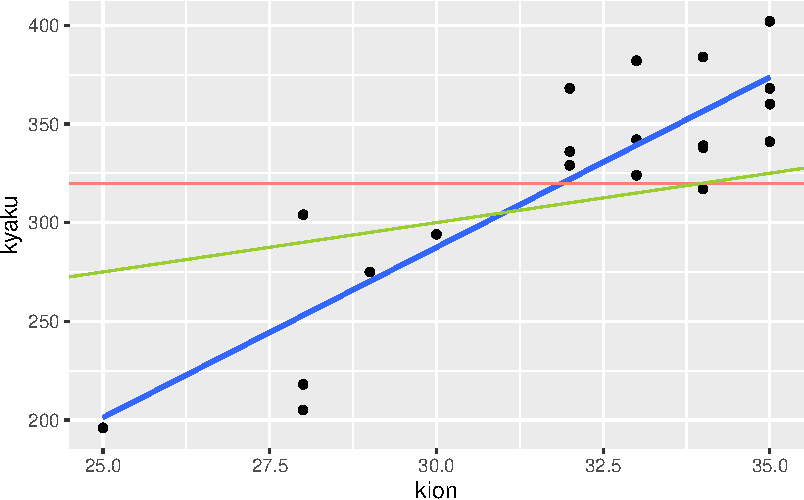
\includegraphics{8_regress_files/figure-pdf/unnamed-chunk-4-1.pdf}

}

\end{figure}

じゃあ,どんな線が最も良い線なのか,それを決めて線を引く,というか線の式を求めるのが回帰分析です。

\hypertarget{ux56deux5e30ux5206ux6790}{%
\chapter{回帰分析?}\label{ux56deux5e30ux5206ux6790}}

回帰分析では,最小二乗法という方法で計算します。この方法の考え方は

直線と各データの誤差を最小にする線が最も良い線であろう

というものです。

これは,他の図で矢印になっている誤差を全部足したらしたらゼロになる点を探すことを意味します。±打ち消し合うので
\(E(u)=0\) が理想です。

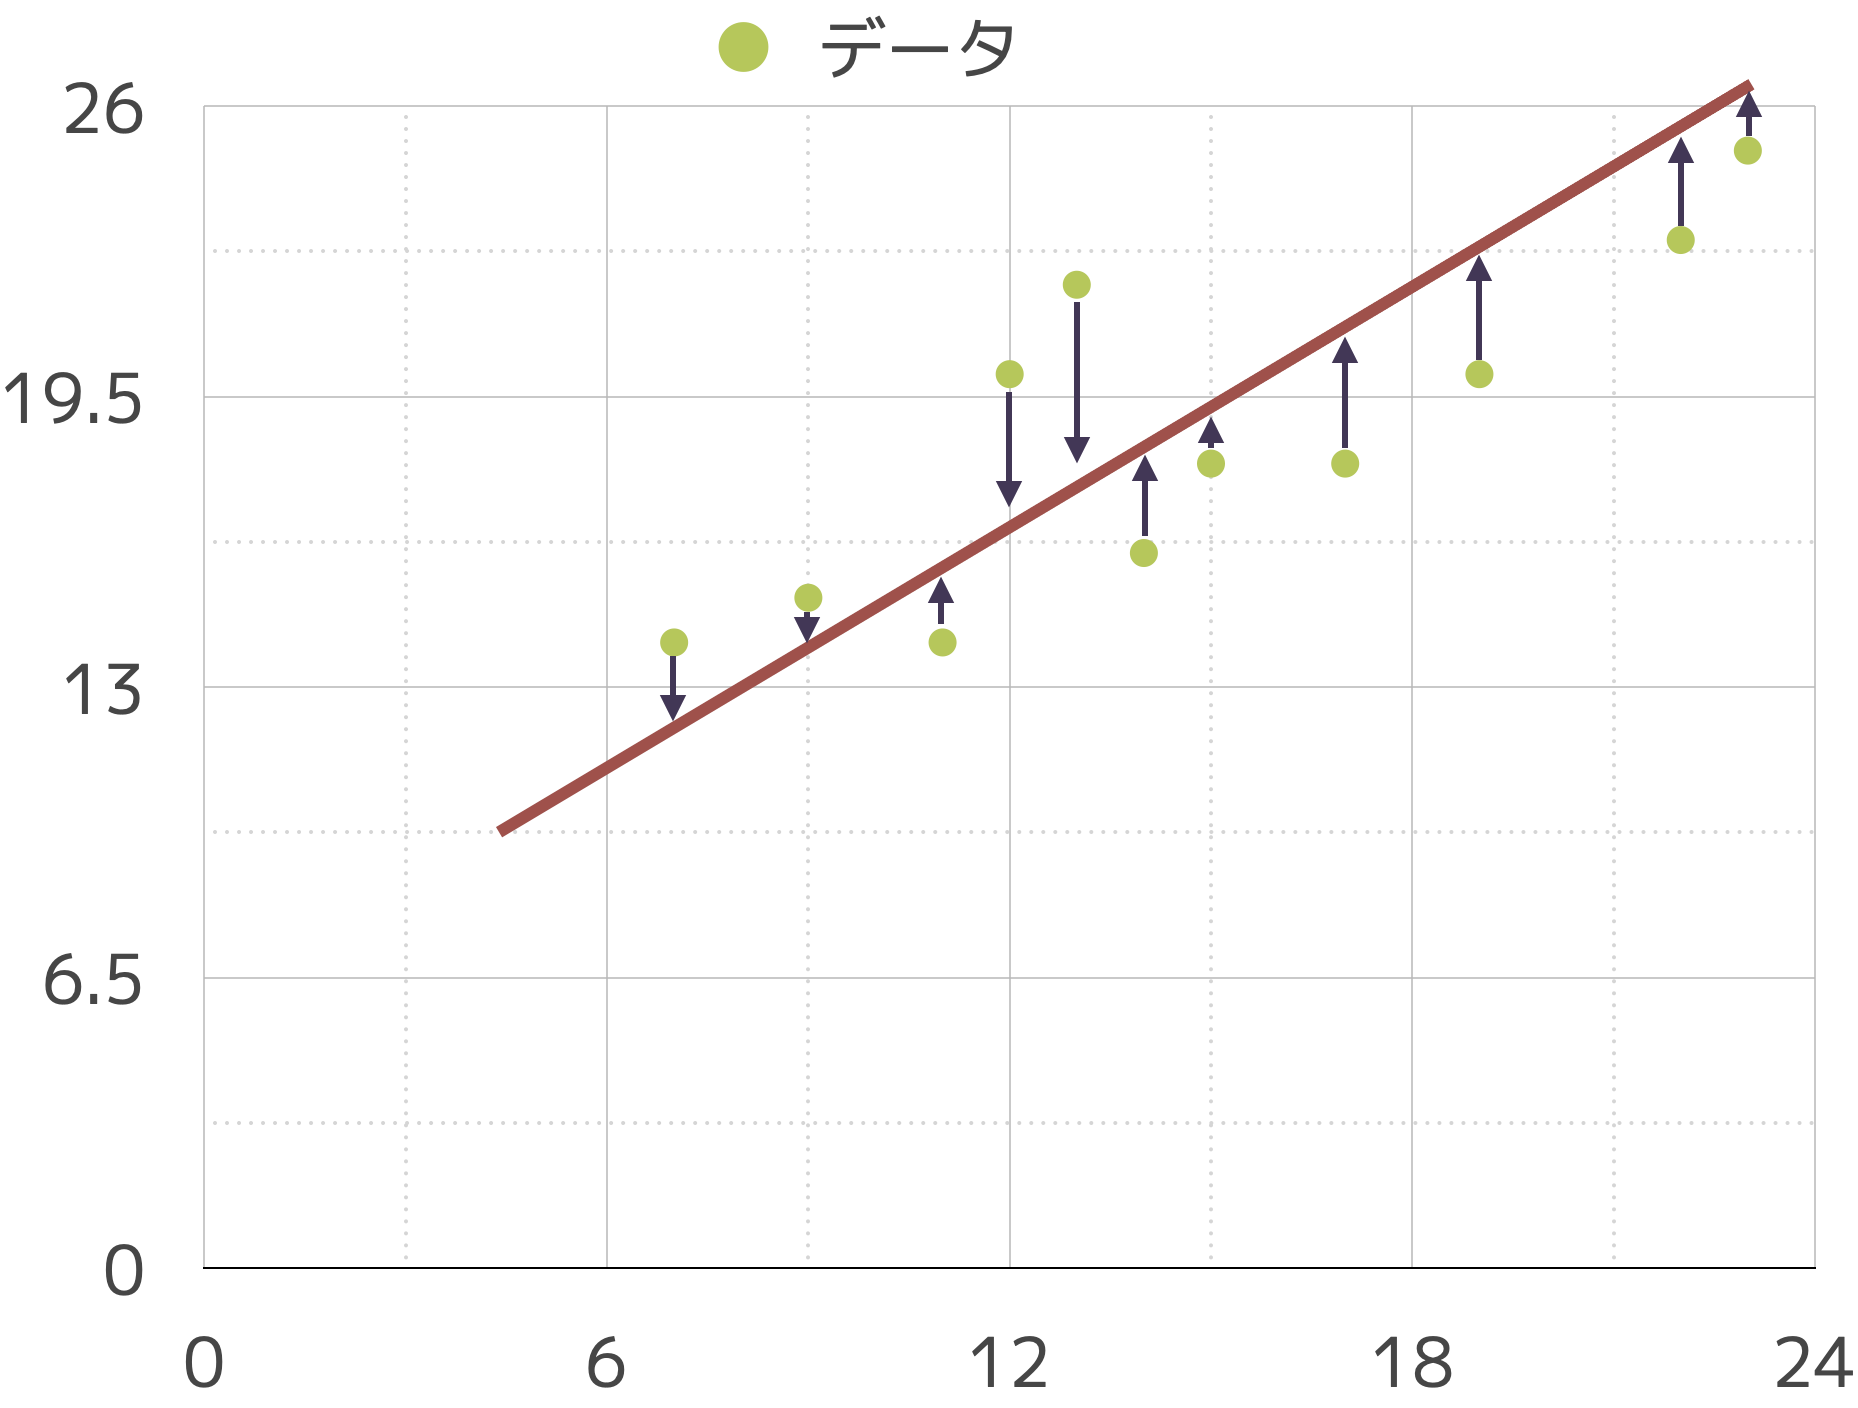
\includegraphics{images/Untitled 2.png}

アイス屋さんにおける気温を\(x\),客数を\(y\)とします。気温とアイスの客数にある一定の傾向があるとは予想できますが,一直線上にビタッと並ぶことはなさそうです。

\begin{itemize}
\tightlist
\item
  近隣で夏祭りがあったら売り上げは伸びるかもしれません
\item
  雨予報が出てたら売り上げは減るかもしれません
\end{itemize}

このような,気温以外の要因で販売量が増減する部分を誤差\(u\)とします。すると

\[
y_i = \beta_0 + \beta_1x_i+u_i
\]

という直線をイメージしていることになります。ただし添え字の\(i\)はサンプル(散布図の個々の点)ですff。誤差が最小になるような線を引きたいので,

\[
u_i = y_i - \beta_0 - \beta_1x_i
\]

が最小となる切片\(\beta_0\)と傾き\(\beta_1\)を探すと良いということです。ということは,絶対としての\(u\)が一番小さくなる,つまり\(|u|=0\)が理想的。ただ,絶対値の計算は少し大変なので,それぞれの残差を2乗したものをすべて足しあわせて,それを最小化すれば良い。

\begin{itemize}
\tightlist
\item
  だから最小二乗法という
\end{itemize}

\hypertarget{ux6700ux5c0fux4e8cux4e57ux6cd5ux3092ux89e3ux304f}{%
\section{最小二乗法を解く}\label{ux6700ux5c0fux4e8cux4e57ux6cd5ux3092ux89e3ux304f}}

数式で表すと

\begin{equation}\protect\hypertarget{eq-8-1}{}{
\sum_{i=1}^n \hat{u}_i^2= \sum_{i=1}^n (y_i -\hat{\beta_0}-\hat{\beta_1}x_1)^2
}\label{eq-8-1}\end{equation}

が最も小さくなる\(\beta_0\)と\(\beta_1\)を求めれば良い。2次関数の最小値問題。微分して0,とすると計算しやすいので,\(\beta_0\)と\(\beta_1\)をそれそれ微分\footnote{バラバラにして微分してまとめ直してもできますが,合成関数の微分の考え方を知ってると即座に計算できます。}して

\begin{equation}\protect\hypertarget{eq-8-2}{}{
\begin{equation}\left\{ \,    \begin{aligned}&\frac{\partial \Sigma}{\partial \hat{\beta_0}} = \sum_{i=1}^n (y_i -\hat{\beta_0}-\hat{\beta_1}x_1) = 0 \\&\frac{\partial \Sigma}{\partial \hat{\beta_1}} = \sum_{i=1}^n x_i(y_i -\hat{\beta_0}-\hat{\beta_1}x_1) = 0  \end{aligned}\right.\end{equation}
}\label{eq-8-2}\end{equation}

という連立方程式を解けば良い。

\begin{tcolorbox}[enhanced jigsaw, opacityback=0, titlerule=0mm, opacitybacktitle=0.6, rightrule=.15mm, coltitle=black, toprule=.15mm, left=2mm, title=\textcolor{quarto-callout-note-color}{\faInfo}\hspace{0.5em}{ヒント}, bottomrule=.15mm, leftrule=.75mm, breakable, toptitle=1mm, colframe=quarto-callout-note-color-frame, colbacktitle=quarto-callout-note-color!10!white, colback=white, arc=.35mm, bottomtitle=1mm]

\(\bar{x}=\dfrac{1}{n}\sum_{i=1}^nx_i\)とする

\begin{enumerate}
\def\labelenumi{\arabic{enumi}.}
\tightlist
\item
  \(\Sigma^n_{i=1}x_i(x_i-\bar x) = \Sigma^n_{i=1}(x_i-\bar x)(x_i-\bar x)\)\footnotemark{}
\item
  \(\Sigma^n_{i=1}y_i(x_i-\bar x) = \Sigma^n_{i=1}x_i(y_i-\bar y) = \Sigma^n_{i=1}(x_i-\bar x)(y_i-\bar y)\)
\end{enumerate}

\end{tcolorbox}

\footnotetext{\[
\begin{split}
\Sigma^n_{i=1}&x_i(x_i-\bar x)  \\
& = \Sigma^n_{i=1} x_i^2 - \bar x \Sigma^n_{i=1} x_i \\
& = \Sigma^n_{i=1}x_i^2 - n(\bar x)^2
\end{split}
\]

一方で

\[
\begin{split}
\Sigma^n_{i=1}&(x_i-\bar x)(x_i-\bar x)  \\
& = \Sigma^n_{i=1} (x_i^2 - 2 x_i \bar x +(\bar x)^2) \\
& = \Sigma^n_{i=1}x_i^2 -2 \bar x \Sigma^n_{i=1}x_i + (\bar x)^2\\
& = \Sigma^n_{i=1}x_i^2 - n(\bar x)^2 \\
\end{split}
\]}

\begin{equation}\protect\hypertarget{eq-8-3}{}{
\begin{equation} 
\left\{ \,   
\begin{split}
&\sum_{i=1}^n (y_i -\hat{\beta_0}-\hat{\beta_1}x_1) = 0  \\
&\sum_{i=1}^n x_i(y_i -\hat{\beta_0}-\hat{\beta_1}x_1) = 0  
\end{split}
\right.
\end{equation}
}\label{eq-8-3}\end{equation}

上の式から

\(\begin{split}&\Sigma y_i - n \hat{\beta_0} - \hat{\beta_1}\Sigma x_i = 0 \\\hat{\beta_0} &= \frac{1}{n} (\Sigma y_i - \hat{\beta_1}\Sigma x_i) \\&= \bar{y} - \hat{\beta_1} \bar{x}\end{split}\)

下の式に代入

\(\begin{split}\Sigma x_i \{y_i - (\bar{y} - \hat{\beta_1}\bar{x}) - \hat{\beta_1}x_i\} &= 0 \\ \Sigma x_i \{(y_i - \bar{y}) - \hat{\beta_1}(x_i - \bar{x})\} &= 0 \\\Sigma x_i (y_i - \bar{y}) - \hat{\beta_1}\Sigma x_i (x_i - \bar{x}) &= 0 \\\end{split}\)

ヒントから

\(\Sigma (x_i - \bar{x})(y_i - \bar{y}) - \hat{\beta_1}\Sigma (x_i - \bar{x}) (x_i - \bar{x}) = 0\)

\begin{equation}\protect\hypertarget{eq-8-4}{}{
\hat{\beta_1} = \dfrac{\Sigma (x_i - \bar{x})(y_i - \bar{y})}{ \Sigma  (x_i - \bar{x})^2} = \dfrac{ x \mbox{と}y\mbox{の共分散}}{ x\mbox{の分散}}
}\label{eq-8-4}\end{equation}

\begin{equation}\protect\hypertarget{eq-8-5}{}{
\hat{\beta_0} = \bar{y} - \dfrac{\Sigma (x_i - \bar{x})(y_i - \bar{y})}{ \Sigma  (x_i - \bar{x})^2} \bar{x}
}\label{eq-8-5}\end{equation}

\hypertarget{rux3067ux306eux5206ux6790}{%
\chapter{Rでの分析}\label{rux3067ux306eux5206ux6790}}

次に,Rで回帰分析をします。回帰分析は,\texttt{lm()}でやります。\texttt{()}の中には,\texttt{(従属変数\ \textasciitilde{}\ 独立変数,\ data\ =\ データ名)}という内容を書きます。結果は,summary(分析結果)で出ます。また,論文に書くような結果の表は,\texttt{modelsummary}パッケージの\texttt{msummary}を使うと出力できます。

\begin{Shaded}
\begin{Highlighting}[]
\NormalTok{kekka4\_1 }\OtherTok{\textless{}{-}} \FunctionTok{lm}\NormalTok{(kyaku }\SpecialCharTok{\textasciitilde{}}\NormalTok{ kion, }\AttributeTok{data =}\NormalTok{ ice4\_1)}
\FunctionTok{summary}\NormalTok{(kekka4\_1)}
\end{Highlighting}
\end{Shaded}

\begin{verbatim}

Call:
lm(formula = kyaku ~ kion, data = ice4_1)

Residuals:
    Min      1Q  Median      3Q     Max 
-47.969 -17.709  -1.218  17.413  51.031 

Coefficients:
            Estimate Std. Error t value Pr(>|t|)    
(Intercept)  -229.98      73.79  -3.117  0.00596 ** 
kion           17.25       2.30   7.499 6.08e-07 ***
---
Signif. codes:  0 '***' 0.001 '**' 0.01 '*' 0.05 '.' 0.1 ' ' 1

Residual standard error: 29.54 on 18 degrees of freedom
Multiple R-squared:  0.7575,    Adjusted R-squared:  0.744 
F-statistic: 56.23 on 1 and 18 DF,  p-value: 6.082e-07
\end{verbatim}

\begin{Shaded}
\begin{Highlighting}[]
\FunctionTok{msummary}\NormalTok{(kekka4\_1,}
         \AttributeTok{gof\_omit =} \StringTok{"Log.Lik.|AIC|BIC|RMSE"}\NormalTok{,}
         \AttributeTok{title =} \StringTok{""}\NormalTok{,          }\CommentTok{\# タイトル}
         \AttributeTok{stars =} \ConstantTok{TRUE}\NormalTok{)}
\end{Highlighting}
\end{Shaded}

\begin{table}

\caption{}
\centering
\begin{tabular}[t]{lc}
\toprule
  & (1)\\
\midrule
(Intercept) & \num{-229.982}**\\
 & (\num{73.787})\\
kion & \num{17.248}***\\
 & (\num{2.300})\\
\midrule
Num.Obs. & \num{20}\\
R2 & \num{0.758}\\
R2 Adj. & \num{0.744}\\
F & \num{56.231}\\
\bottomrule
\multicolumn{2}{l}{\rule{0pt}{1em}+ p $<$ 0.1, * p $<$ 0.05, ** p $<$ 0.01, *** p $<$ 0.001}\\
\end{tabular}
\end{table}

\hypertarget{ux56deux5e30ux5206ux6790ux306bux304aux3051ux308bux4eeeux8aacux691cux5b9a}{%
\chapter{回帰分析における仮説検定}\label{ux56deux5e30ux5206ux6790ux306bux304aux3051ux308bux4eeeux8aacux691cux5b9a}}

回帰分析は,未知の母集団における法則性を推定しています。

\begin{itemize}
\tightlist
\item
  例えば,アイス屋さんの気温と客数の関係を推定した前項の分析は,ある期間(例えば2023年8月)の関係を見ているとします。
\item
  しかし,この分析から知りたいのは,2023年の関係だけではなく,もっと一般的な基本と客数の関係です。

  \begin{itemize}
  \tightlist
  \item
    例えば来年以降の8月はどうか,など
  \end{itemize}
\item
  ここから,上の回帰分析は,ある月(データの取り方によっては特定の月ではなく一般に)アイスクリーム屋さんにとって気温と客数の関係はどんなものかを母集団としていると考えられます。
\end{itemize}

少ないデータによって未知の母集団を推定しているので,その推定値は 必ずしも母集団と一致するわけではありません。

そこで,この母集団を推定するにあたっての性能を統計的に検定することが一般的です。

具体的には,係数が0(つまり関係ない)かどうかを平均値の差の検定と同じt検定で検定します。

詳しいことは割愛しますが,帰無仮説を0とおいたt検定の結果が,先ほどの回帰式でいうt
valueとして表示されていて,有意確率が
Pr(\textgreater\textbar t\textbar)として表示されています。

\begin{Shaded}
\begin{Highlighting}[]
\FunctionTok{lm}\NormalTok{(kyaku }\SpecialCharTok{\textasciitilde{}}\NormalTok{ kion, }\AttributeTok{data =}\NormalTok{ ice4\_1) }\SpecialCharTok{\%\textgreater{}\%} 
  \FunctionTok{summary}\NormalTok{()}
\end{Highlighting}
\end{Shaded}

\begin{verbatim}

Call:
lm(formula = kyaku ~ kion, data = ice4_1)

Residuals:
    Min      1Q  Median      3Q     Max 
-47.969 -17.709  -1.218  17.413  51.031 

Coefficients:
            Estimate Std. Error t value Pr(>|t|)    
(Intercept)  -229.98      73.79  -3.117  0.00596 ** 
kion           17.25       2.30   7.499 6.08e-07 ***
---
Signif. codes:  0 '***' 0.001 '**' 0.01 '*' 0.05 '.' 0.1 ' ' 1

Residual standard error: 29.54 on 18 degrees of freedom
Multiple R-squared:  0.7575,    Adjusted R-squared:  0.744 
F-statistic: 56.23 on 1 and 18 DF,  p-value: 6.082e-07
\end{verbatim}

気温(
\texttt{kion})の係数は17.25,有意確率は限りなく0に近い(気温と客数に関係がないとする仮説は99.999)

\hypertarget{ux901aux904eux30c6ux30b9ux30c8}{%
\section{通過テスト}\label{ux901aux904eux30c6ux30b9ux30c8}}

\begin{Shaded}
\begin{Highlighting}[]
\NormalTok{ice4\_9 }\OtherTok{\textless{}{-}} \FunctionTok{read\_csv}\NormalTok{(}\StringTok{"data/ice1\_9.csv"}\NormalTok{)}



\FunctionTok{lm}\NormalTok{(gpa }\SpecialCharTok{\textasciitilde{}}\NormalTok{ exam, }\AttributeTok{data =}\NormalTok{ ice4\_9) }\OtherTok{{-}\textgreater{}}\NormalTok{ kekka}


\FunctionTok{msummary}\NormalTok{(kekka,}
         \AttributeTok{gof\_omit =} \StringTok{"Log.Lik.|AIC|BIC"}\NormalTok{,}
         \AttributeTok{title =} \StringTok{""}\NormalTok{,          }\CommentTok{\# タイトル}
         \AttributeTok{stars =} \ConstantTok{TRUE}\NormalTok{)}
\end{Highlighting}
\end{Shaded}

\begin{table}

\caption{}
\centering
\begin{tabular}[t]{lc}
\toprule
  & (1)\\
\midrule
(Intercept) & \num{-1.797}+\\
 & (\num{0.896})\\
exam & \num{0.008}***\\
 & (\num{0.002})\\
\midrule
Num.Obs. & \num{19}\\
R2 & \num{0.580}\\
R2 Adj. & \num{0.556}\\
F & \num{23.509}\\
RMSE & \num{0.48}\\
\bottomrule
\multicolumn{2}{l}{\rule{0pt}{1em}+ p $<$ 0.1, * p $<$ 0.05, ** p $<$ 0.01, *** p $<$ 0.001}\\
\end{tabular}
\end{table}

\begin{Shaded}
\begin{Highlighting}[]
\CommentTok{\# 予測値の作成}
\NormalTok{newdata }\OtherTok{\textless{}{-}} \FunctionTok{tibble}\NormalTok{(}\AttributeTok{exam =} \FunctionTok{c}\NormalTok{(}\DecValTok{400}\NormalTok{,}\DecValTok{500}\NormalTok{,}\DecValTok{600}\NormalTok{,}\DecValTok{700}\NormalTok{))}
\FunctionTok{predict}\NormalTok{(kekka,}\AttributeTok{new =}\NormalTok{ newdata)}
\end{Highlighting}
\end{Shaded}

\begin{verbatim}
       1        2        3        4 
1.429565 2.236329 3.043092 3.849855 
\end{verbatim}



\end{document}
